\documentclass{article}

\usepackage[margin=0.75in]{geometry}
\usepackage{graphicx}
\usepackage{subcaption}
\usepackage{emoji}

\begin{titlepage}
    \title{IDATT2202, Assignment 4}
    \author{Jakob Grønhaug (jakobkg@stud.ntnu.no)}
\end{titlepage}

\begin{document}
\maketitle

\section{File systems}

\begin{enumerate}
    \item \textbf{Design factors}

          Two important factors in the design of a file system are capacity and performance.

          Capacity in the context of a file system refers to the ratio of total physical storage available on a device to user accessible storage in the file system. A file system can use up some of the available physical storage for itself, allocating it to metadata of various kinds of metadata instead of making it accessible to the rest of the system. Different types of file systems reserve different amounts of data to itself, with some file systems needing multiple physical disks and only making the capacity of one disk accessible to the rest of the system, reserving the rest for redundant copies of data to ensure data is not lost even in the case of a hardware failure (Redundant Array of Independent Disks or RAID).

          Performance in a file system is often thought of in terms of response time (the time it takes from data is requested until the first byte arrives) and throughput (number of bits or bytes read per unit of time under various conditions). A user would want a program to start or a file to be opened without significant waiting times after selecting them in their interface, and should also be allowed to expect throughput that doesn't hinder their experience. The largest recent improvements in response times have come from improvements in hardware rather than software, as we have moved at a rapid pace from magnetic disks with mechanical components to purely electrical storage that does not need to wait for a disk to spin up or an arm to move into position before it can start providing the requested data.

    \item \textbf{Metadata}

          File metadata is "sidecar" data describing the actual data contained in the file, such as file size, when the file was last changed and what users/groups on the system have what sorts of access to the file (read/write/execute are often used).
\end{enumerate}

\section{Files and directories}

\begin{enumerate}
    \item \textbf{FFS}
          \begin{enumerate}
              \item \textbf{Hard and soft links}

                    Hard links are direct mappings between a file name and the underlying data in the file system, while soft links (aka symbolic links) are references to hard links.

                    \begin{figure}[ht]
                        \centering
                        \begin{subfigure}{.45\textwidth}
                            \centering
                            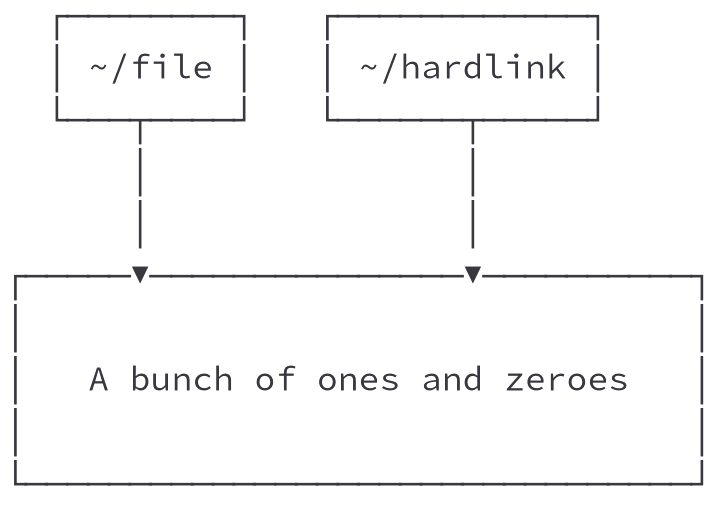
\includegraphics[width=.8\linewidth]{illustrasjoner/hardlink.png}
                            \caption{A file with a hard link to it}
                        \end{subfigure}
                        \begin{subfigure}{.45\textwidth}
                            \centering
                            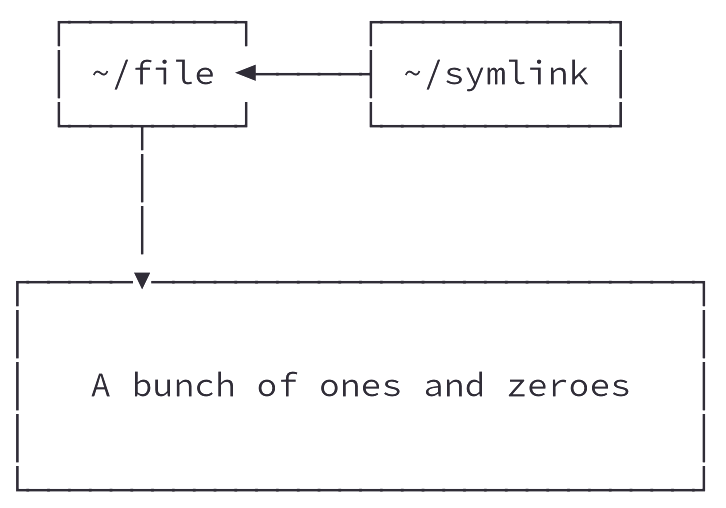
\includegraphics[width=.8\linewidth]{illustrasjoner/symlink.png}
                            \caption{A file with a soft link to it}
                        \end{subfigure}
                        \caption{The difference between hard links and soft links (aka symlinks)}
                    \end{figure}

                    In an ext4 file system, a soft link file is one block of data (e.g. 4KB).

              \item \textbf{Minimum number of references for any folder}

                    Any folder must contain references to itself (\verb+.+) and its parent (\verb+..+).
              \item \textbf{Folder w/ five subfolders}

                    A folder with five subfolders appears to only have one hard link
                    \begin{verbatim}
> ls tmp
1  2  3  4  5

> ls -ld tmp
drwxr-xr-x. 1 jakob jakob 10 Nov 15 12:41 tmp
                \end{verbatim}
              \item \textbf{Spatial locality}

                    In FFS like ext4, spatial locality is achieved by grouping data blocks on disk into groups, and attempting to ensure that a directory's data blocks and metadata blocks are always within the same block group.

          \end{enumerate}
    \item \textbf{NTFS}
          \begin{enumerate}
              \item \textbf{Resident/non-resident attributes}

                    In NTFS, a resident attribute is an attribute whose contents are stored directly in the master file table while a non-resident attribute is one where an extent pointer is stored in the master file table and the actual contents are stored in said extent.

                    Typically, metadata is small enough to be stored in resident attributes. In NTFS the actual data of a file is just another attribute in the table, and will be stored in a resident attribute for a sufficiently tiny file and in a non-resident attribute for larger files.

              \item \textbf{Extents vs blocks}

                    The variable sized extents used in NTFS allow some flexibility and optimization over the fixed-size blocks seen in FFS. Where FFS uses multiple blocks and handles references with various degrees of separation (indirect blocks), NTFS can keep things simpler with single extents of the needed size. However, the allocation strategy of NTFS causes internal fragmentation issues which has caused the need for "defragmentation utilities" to be included with Windows. This issue is not present in other files systems, and as such FFS based Linux distributions do not need equivalent utilities.
          \end{enumerate}

    \item \textbf{Copy-on-write}

          Copy-on-write helps protect against data corruption by eliminating the possibility of an interrupted write leaving a file in an invalid state. Rather than overwriting the existing copy of a file when writing to it, COW file systems create a new copy of the file with the new contents, meaning that if the process writing to the file is halted for any reason, the previous version of the file is fully intact and untouched.
\end{enumerate}

\section{Security}

\begin{enumerate}
    \item \textbf{Authentication}
          \begin{enumerate}
              \item \textbf{Salt} \emoji{salt}

                    Hashing passwords with an unique salt helps mitigate a class of attacks where an adversary is able to access the database of hashed passwords to a system. If the hashing algorithm is known, the attacker will then be able to run any number of potential passwords through said hashing algorithm and check the password database for matching hashes. Since there is a relatively limited number of hashing algorithms in use for such purposes, attackers may even have a precomputed database of hashes to compare against. Adding a salt to the hashing process foils this type of attack, as it's no longer feasible to just look in a precomputed password/hash table for potential matches.

              \item \textbf{Updating a file that you do not have permissions to}

                    A user could be able to update the password database without having access to it by using a setuid program, meaning a program that runs with a different set of permissions than those of whoever is currently executing it. This still requires the setuid program and its author to be trusted, but this seems to me to be a far smaller risk to take than to allow users read/write access to the password database of a system.
          \end{enumerate}

    \item \textbf{Software vulnerabilities}
          \begin{enumerate}
              \item \textbf{The problem with} \verb+gets()+

                    The \verb+gets()+ library call takes a user controlled input and places it into a location given by a pointer without first verifying whether the provided input actually fits within the allocated space at said pointer or not. This allows for a myriad of different attacks where a properly crafted input will overflow the boundaries of the allocated space and overwrite other data. If the pointer given points to a location on the stack, \verb+gets()+ will happily write its way into the return pointer at the top of the stack which further opens the gates for an attacker to control code execution.

                    This is mitigated by using different calls with similar functionality that allow the programmer to limit the amount of data copied such as \verb+scanf()+ or \verb+fgets()+.
            
            \item \textbf{Microkernel vs monolithic kernel}
            
                A microkernel design is one where the kernel itself is kept as small as possible by running as much of it as possible in user-level servers. For example, in Linux systems today parts of the system is designed using a microkernel approach. For example, the display/window manager is not part of the kernel itself and is instead ran as a user mode server. This approach reduces the attack surface of the kernel which results in statistically increased security, and the increased modularity of the system allows more user freedom in choosing different components for their system (see: X11 vs Wayland as Linux display servers, or the myriad of window managers out there).
          \end{enumerate}
\end{enumerate}


\end{document}